\providecommand{\pdfxopts}{a-1b,cyrxmp}
\providecommand{\thisyear}{2020}
\immediate\write18{rm \jobname.xmpdata}%  uncomment for Unix-based systems
\begin{filecontents*}{\jobname.xmpdata}
\Title{Силовая электроника. Виртуальная лабораторная работа №2\textemdash\thisyear}
\Author{Артем Николаевич Прокшин}
\Creator{pdfTeX + pdfx.sty with options \pdfxopts }
\Subject{Виртуальная лабораторная работа №2
\sep
исследование неуправляемых
\sep
выпрямителей и фильтров
\sep
выпрямленного тока}
\Keywords{неуправляемый выпрямитель, фильтры, ЛЭТИ}
\CoverDisplayDate{апрель \thisyear}
\CoverDate{2020-04-04}
\Copyrighted{True}
\Copyright{Public Domain}
\CopyrightURL{http://github.com/trot-t}
\Creator{pdfTeX + pdfx.sty with options \pdfxopts }
\end{filecontents*}

\documentclass[a4paper,12pt]{article}

\pdfcompresslevel=9

\usepackage[\pdfxopts]{pdfx}[2016/04/04]
\PassOptionsToPackage{obeyspaces}{url}
\let\tldocrussian=1  % for live4ht.cfg


\usepackage{extsizes} 
\usepackage[left=10mm, top=20mm, right=10mm, bottom=20mm, nohead, footskip=7mm]{geometry} % настройки полей документа


\usepackage[T2A]{fontenc}
\usepackage[utf8]{inputenc}
\usepackage[english,russian]{babel}
\usepackage{tikz}
\usetikzlibrary{positioning}
\usepackage[european,cuteinductors,smartlabels,siunitx]{circuitikz}

%%% Межстрочный интервал
\usepackage{setspace}

%% таблицы
\usepackage{booktabs}
%multi-row
\usepackage{multirow}

%% для кода
\usepackage{color}
\usepackage{listingsutf8}

%\input{colors}
\definecolor{lightgrey}{rgb}{0.9,0.9,0.9}
\definecolor{lightblue}{rgb}{0,0,1}

\definecolor{grey}{rgb}{0.5,0.5,0.5}
\definecolor{blue}{rgb}{0,0,1}
\definecolor{violet}{rgb}{0.5,0,0.5}

\definecolor{darkred}{rgb}{0.5,0,0}
\definecolor{darkblue}{rgb}{0,0,0.5}
\definecolor{darkgreen}{rgb}{0,0.5,0}


\lstset{%
  language=C++,%
  morekeywords={constexpr,nullptr,size_t,uint32_t,assert,override,final},%
  basicstyle=\ttfamily\footnotesize,%
  sensitive=true,%
  keywordstyle=\color{blue},%
  stringstyle=\color{darkgreen},%
  commentstyle=\color{violet},%
  showstringspaces=false,%
  tabsize=2,%
  frame=leftline,
  rulecolor=\color{lightblue},
  xleftmargin=20pt,
}

\lstset{
%extendedchars=\true,
%inputencoding=utf8x,   
  numberstyle=\tiny,
  numbers=left,
  numbersep=10pt,
  xleftmargin=20pt,
  %framesep=4.5mm,
  %framexleftmargin=2.5mm,
  framexleftmargin=5pt,
  framesep=15pt,
  fillcolor=\color{lightgrey},
}


\title{Исследование неуправляемых выпрямителей и фильтров выпрямленного тока}
\author{}
% Конец преамбулы
\begin{document}
%\maketitle
%\begin{tikzpicture}
%\newcommand{\xb}{-3}
%\newcommand{\xa}{3}
%\draw[thin, ->] (-6,0) -- (6,0) node[right] {$X$};
%\draw[thin, ->] (0,-6) -- (0,6) node[left] {$Y$};
%\foreach \x\xtext in {-5/-5,5/5,{\xb}/\xb,{\xa}/{\displaystyle \frac{-b+\sqrt{b^2-4ac}}{2a}}} % 
%   \draw (\x,0.1) -- (\x,-0.1) node[below] {$\xtext$};

 %\draw[domain=-5:5, help lines, smooth]
 %       plot ({\x},{0.2*(\x-\xa)*(\x-\xb)});
%\end{tikzpicture}
%\section{Прецизионные схемы и малошумящая аппаратура}
\section{Исследование неуправляемых выпрямителей и фильтров выпрямленного тока}

{\bf Целью} работы является исследование характеристик различных вариантов схем неуправляемых выпрямителей однофазного напряжения 
и влияние на их работу сглаживающих фильтров.
 
\subsection{Виртуальная установка для исследования свойств неуправляемых выпрямителей} 

\begin{figure}[!ht]
\centering
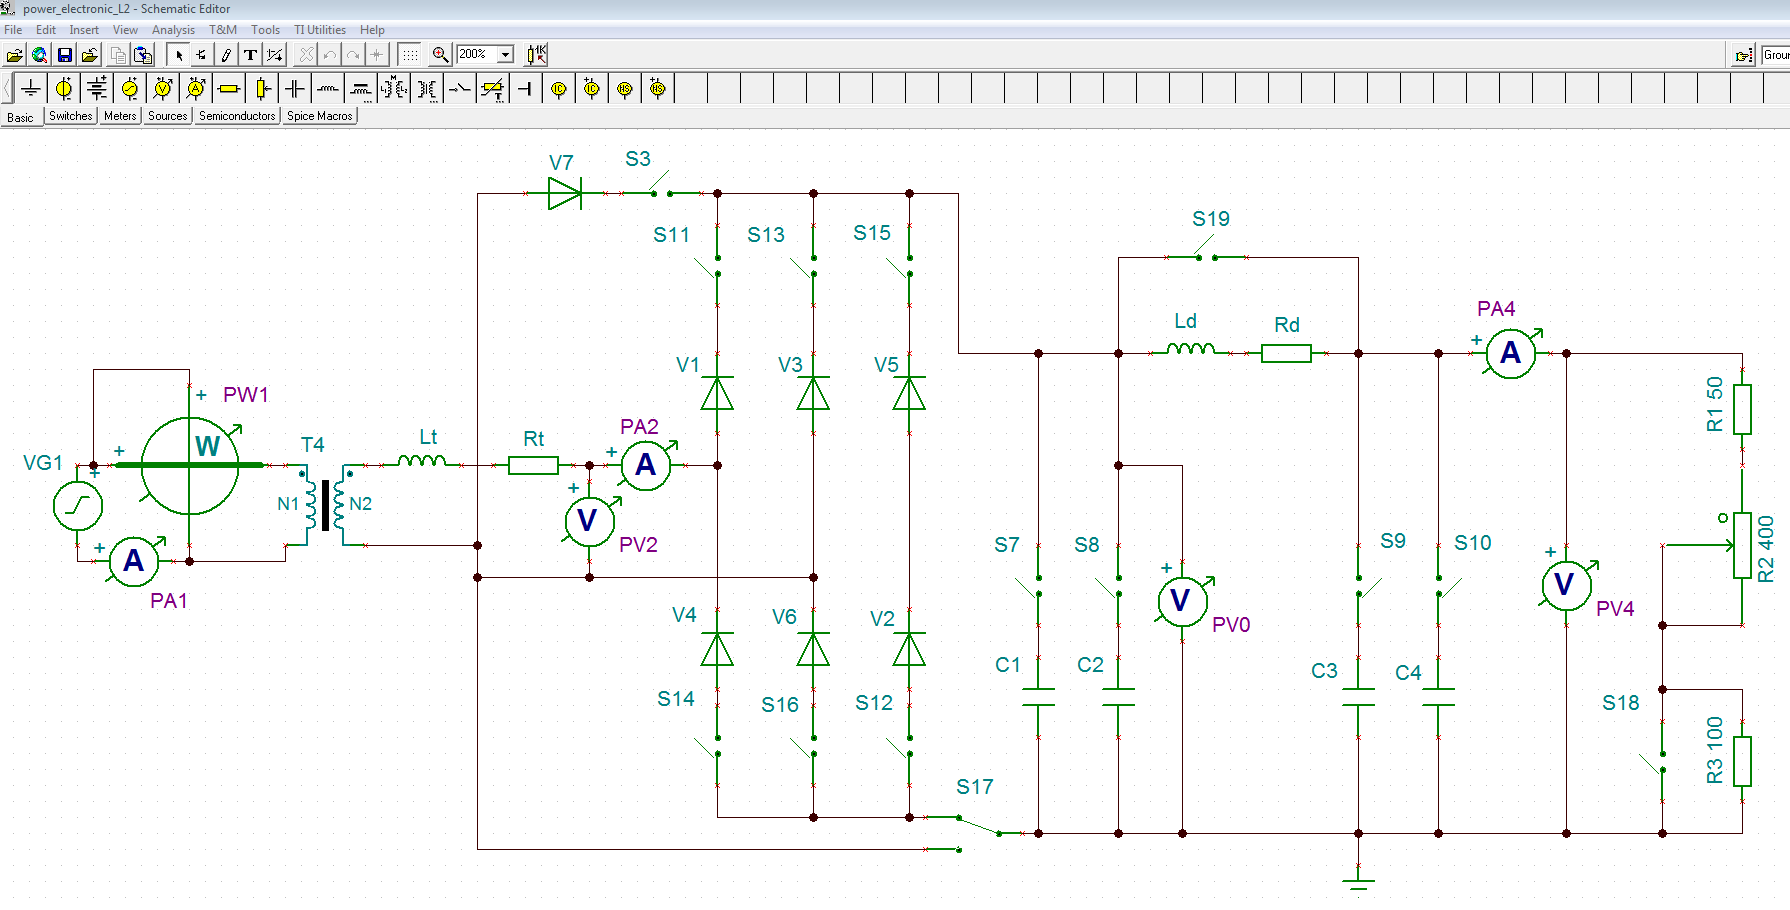
\includegraphics[scale=0.4, angle=90]{setup_lab2}
\caption{схема виртуальной установки для исследования свойств неуправляемых выпрямителей}
\label{setup}
\end{figure}

Виртуальная установка представленная на схеме \ref{setup} запускается с помощью программы \href{http://www.ti.com/tool/TINA-TI}{tina} с бесплатной лицензией.

На виртуальной установке с помощью тумблеров можно исследовать следующие схемы выпрямителей:

\begin{itemize}
\item однофазную однополупериодную;
\item однофазную однополупериодную с шунтирующим диодом;
\item однофазную мостовую.
\end{itemize}

Далее следовать методике описанной в \href{https://github.com/trot-t/power_el_method_old/blob/master/%D0%A1%D0%B8%D0%BB%D0%BE%D0%B2%D0%B0%D1%8F%20%D1%8D%D0%BB%D0%B5%D0%BA%D1%82%D1%80%D0%BE%D0%BD%D0%B8%D0%BA%D0%B0%20%D0%BC%D0%B5%D1%82%D0%BE%D0%B4%D0%B8%D1%87%D0%BA%D0%B0%20%D0%BB%D0%B0%D0%B1%D0%BE%D1%80%D0%B0%D1%82%D0%BE%D1%80%D0%BD%D1%8B%D0%B5.pdf}{методичке} для реальной лабораторной установке.


\subsection{порядок выполнения измерений на виртуальной установке}

\begin{itemize}
	\item Открыть \href{https://github.com/trot-t/power_electronics_virtual_labs/blob/master/power_electronic_L2.TSC}{схему} в программе tina;
\item С помощью тумблеров $S_3,S_{11},S_{13},S_{14},S_{16}, S_{17}$ составить схему выпрямителя, указанную преподавателем;
\item Выбрать в меню анализ $\Rightarrow$ переходных процессов (transient analisys) $\Rightarrow$ для нескольких периодов колебаний 
	входной сети, 
	например, с момента времени 40 мс до 100 мс.
\begin{figure}[!ht]
\centering
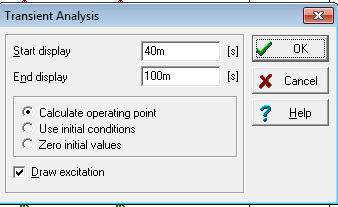
\includegraphics[scale=0.4]{analisys}
\caption{анализ переходных процессов}
\label{analisys}
\end{figure}	

\item получаем мгновенные значения для токов и напряжений вида 
\begin{figure}[!ht]
\centering
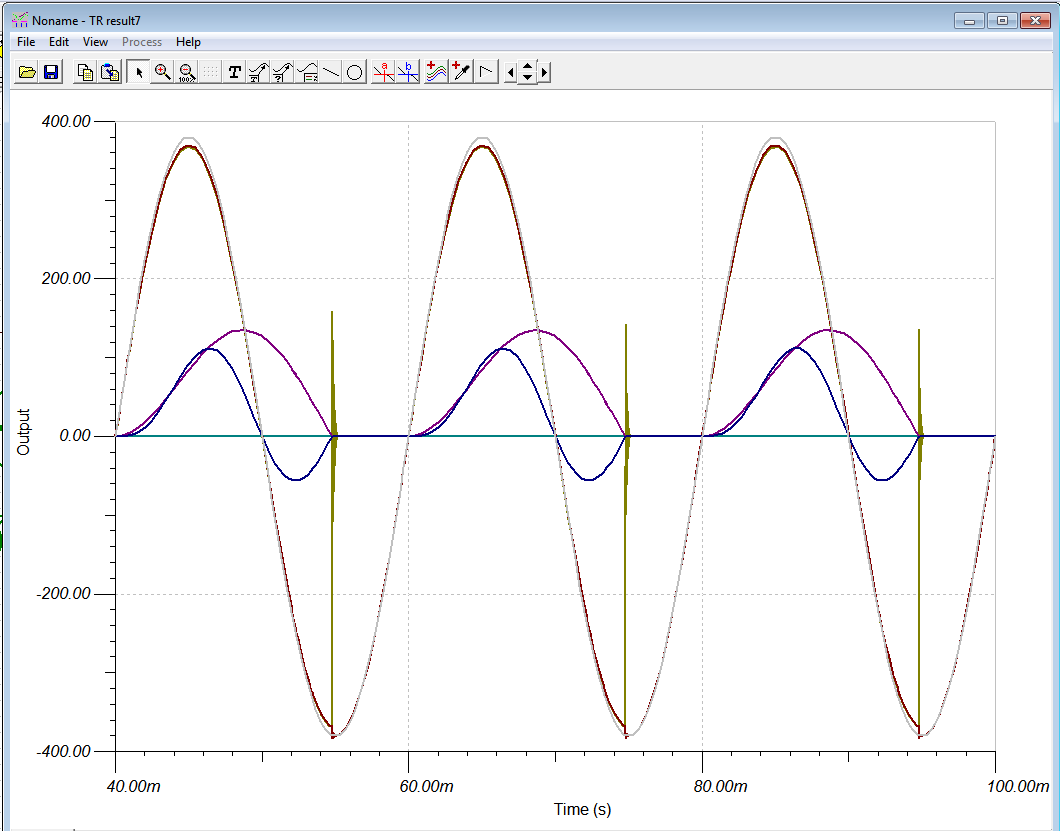
\includegraphics[scale=0.3]{result}
\caption{результат анализа переходных процессов}
\label{result}
\end{figure}	

\item Можно отобразить отдельную кривую <<show/hide curves>>. Также можно разобрать кривые по отдельным графикам. 
	Для этого в меню графика выбрать <<split curves>>
\begin{figure}[!ht]
\centering
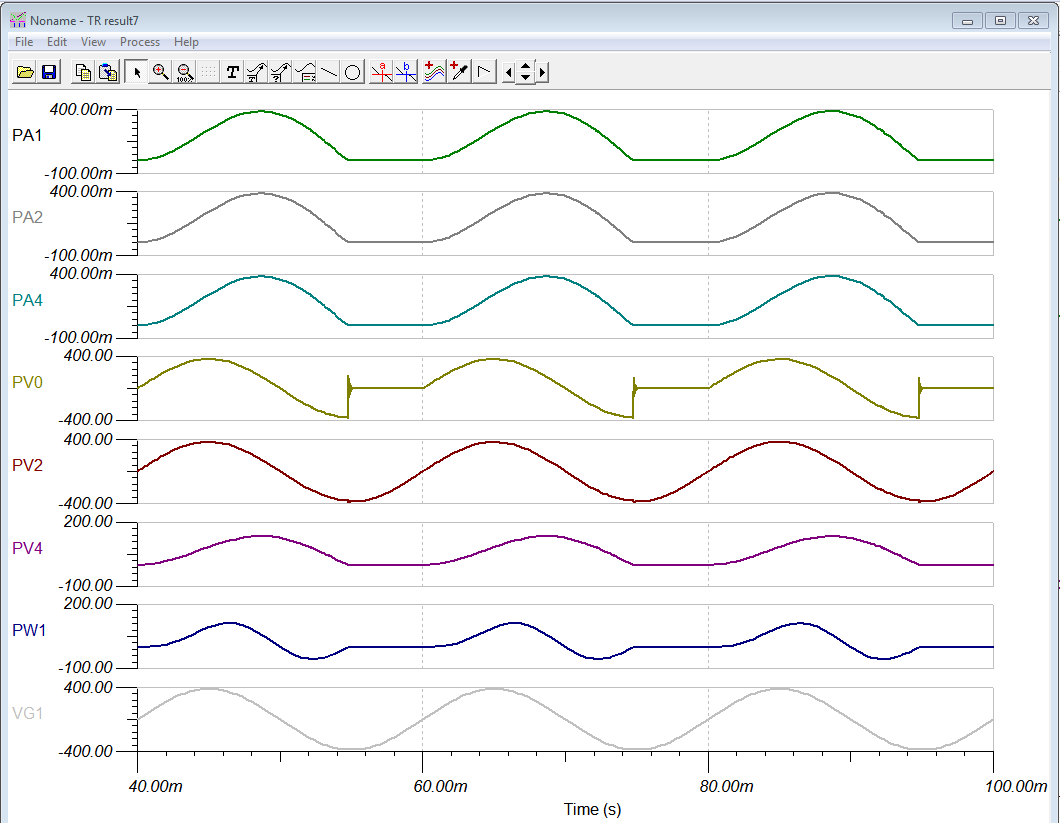
\includegraphics[scale=0.3]{result_splitted}
\caption{графики всех параметров}
\label{result_splitted}
\end{figure}  

\item В реальной установке для измерения действующих значений и средних значений используются приборы с различной
	измерительной системой. В виртуальной установке для получения действующих значений и средних значений
	выбрать график параметра, например, $PV4$ мышью, в меню графика выбрать Process $\Rightarrow$ <<Averages...>>.
\begin{figure}[!ht]
\centering
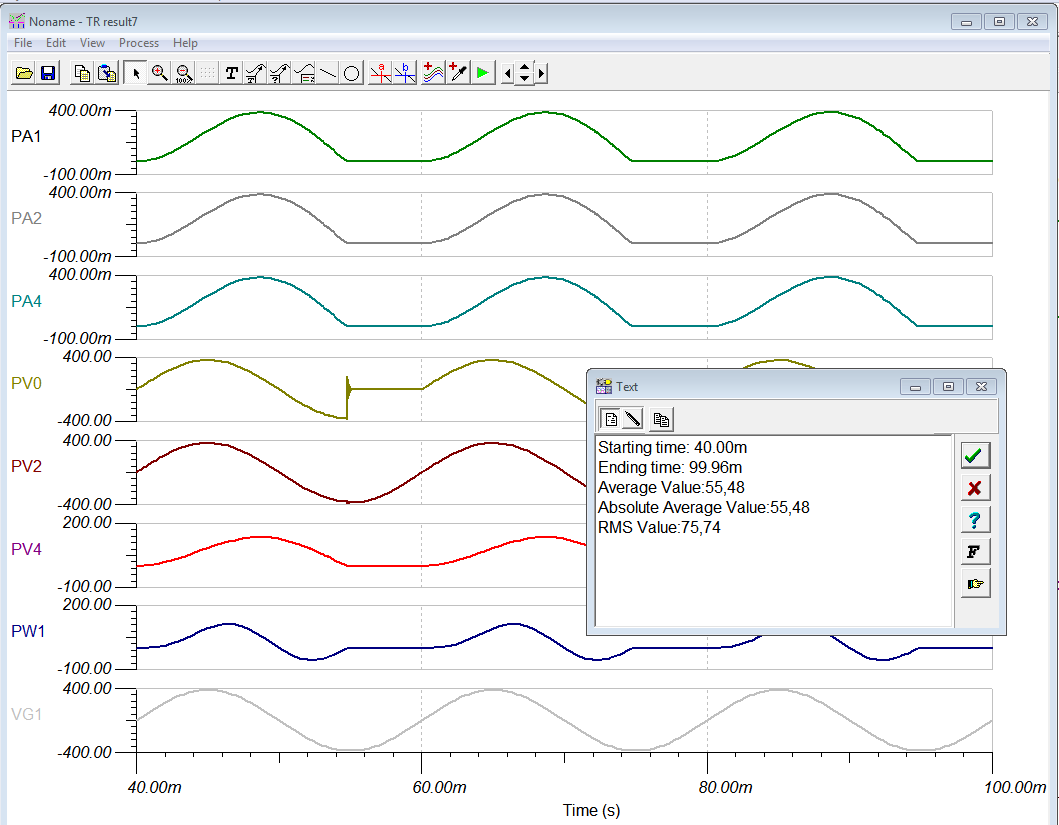
\includegraphics[scale=0.3]{result_rms_avg}
\caption{действующие и средние значения}
\label{result_rms_avg}
\end{figure}

\item параметры дросселя изменять в соответствии с параметрами реальной установки:
\begin{table}[!ht]
\centering
\begin{tabular}{l|l|l}
\toprule
	2-е положение& $L_d$=0,394 Гн& $R_d$= 11 ом \\
\midrule
        3-е положение& $L_d$=0,86 Гн& $R_d$= 19,3 ом \\
\midrule
        4-е положение& $L_d$=2,12 Гн& $R_d$= 29,3 ом \\
\midrule
        5-е положение& $L_d$=4,07 Гн& $R_d$ = 38 ом \\
\bottomrule
\end{tabular}
	\caption{параметры дросселя}
\end{table}

\item прочие параметры также соответствуют параметрам реальной установки:
\begin{table}[!ht]
\centering
\begin{tabular}{lcl}
\toprule
	$R_\textcyrillic{тр}$ &=& 8 ом\\
%\midrule
	$R_\textcyrillic{вентиля динамическое}$ &=& 1,6 ом\\
%\midrule
	$x_a$ &=& 37 ом \\
%\midrule
	$U_\textcyrillic{о.вентиля}$ &=& 0,4 В \\
\bottomrule
\end{tabular}
\caption{Прочие параметры}
\end{table} 
\end{itemize}

%\subsection{фотография реальной установки}
\begin{figure}[!ht]
\centering
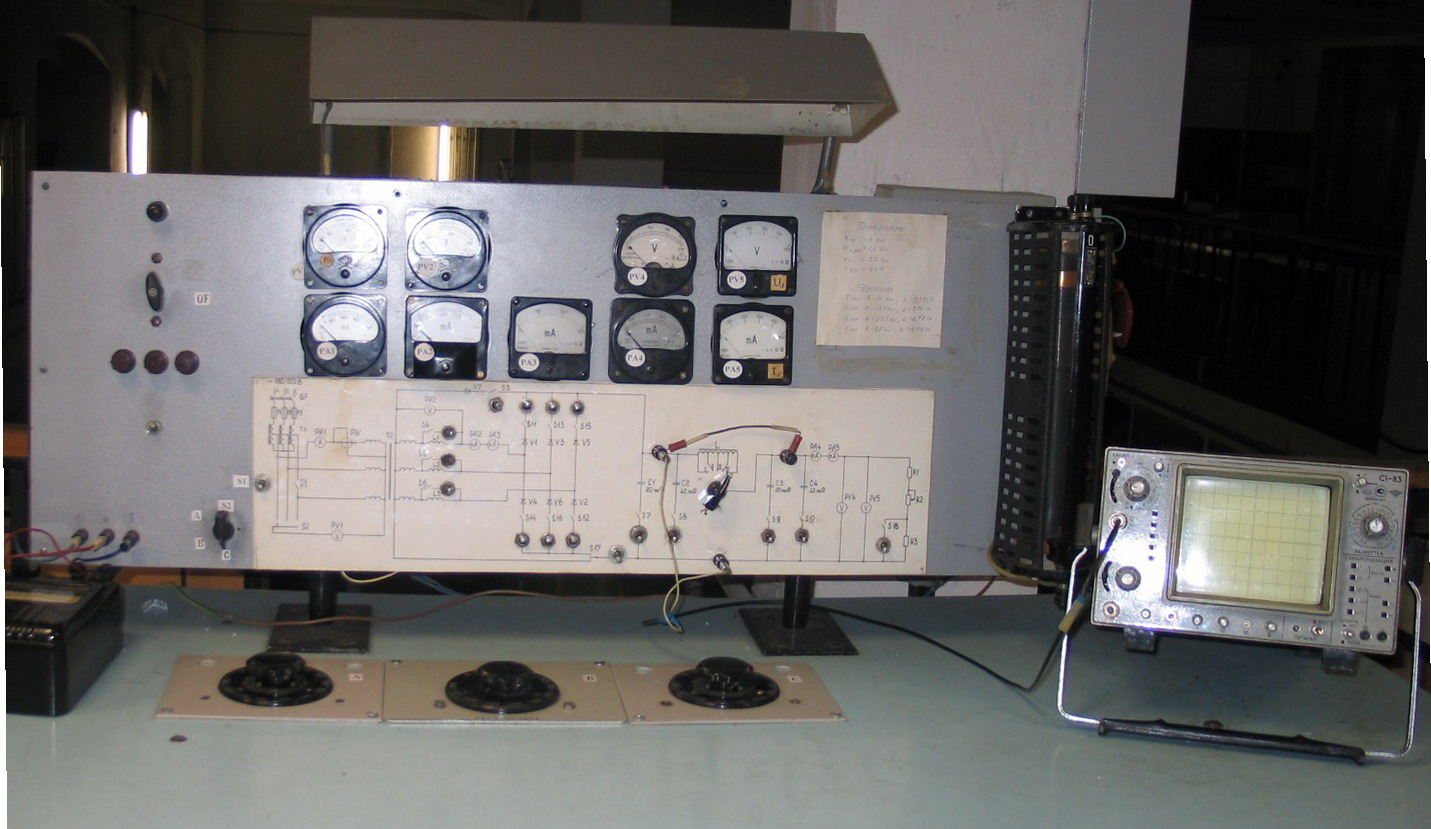
\includegraphics[scale=0.8]{lab2_real}
\caption{фотография реальной установки}
\label{result_rms_avg}
\end{figure}

\end{document}
